

\documentclass[11pt]{article}
\usepackage{acl2015}
\usepackage{times}
\usepackage{latexsym}
% \setlength\titlebox{5cm}    % Expanding the titlebox

%%% Custom additions %%%
% \usepackage{hyperref}
\usepackage{url}
\usepackage[leqno, fleqn]{amsmath}
\usepackage{amssymb}
\usepackage{qtree}
\usepackage{graphicx}
\usepackage{booktabs}
\usepackage{colortbl}
% \usepackage{caption}
\usepackage{subcaption}
\usepackage{color}
\usepackage{xcolor}
\usepackage{tikz}
\usepackage{ifthen}

\newcount\colveccount
\newcommand*\colvec[1]{
        \global\colveccount#1
        \begin{bmatrix}
        \colvecnext
}
\def\colvecnext#1{
        #1
        \global\advance\colveccount-1
        \ifnum\colveccount>0
                \\
                \expandafter\colvecnext
        \else
                \end{bmatrix}
        \fi
}


\newcommand{\nateq}{\equiv}
\newcommand{\natind}{\mathbin{\#}}
%\newcommand{\natneg}{\raisebox{2px}{\tiny\thinspace$\wedge$\thinspace}}
\newcommand{\natneg}{\mathbin{^{\wedge}}}
\newcommand{\natfor}{\sqsubset}
\newcommand{\natrev}{\sqsupset}
\newcommand{\natalt}{\mathbin{|}}
\newcommand{\natcov}{\mathbin{\smallsmile}}

\newcommand{\plneg}{\mathop{\textit{not}}}
\newcommand{\pland}{\mathbin{\textit{and}}}
\newcommand{\plor}{\mathbin{\textit{or}}}

% Strikeout
\newlength{\howlong}\newcommand{\strikeout}[1]{\settowidth{\howlong}{#1}#1\unitlength0.5ex%
\begin{picture}(0,0)\put(0,1){\line(-1,0){\howlong\divide\unitlength}}\end{picture}}

\newcommand{\True}{\texttt{T}}
\newcommand{\False}{\texttt{F}}
\usepackage{stmaryrd}
\newcommand{\sem}[1]{\ensuremath{\llbracket#1\rrbracket}}

\newcommand{\mynote}[1]{{\color{blue}#1}}

\newcommand{\tbchecked}[1]{{\color{red}#1}}

\usepackage{gb4e}
\noautomath

\def\ii#1{\textit{#1}}
\newcommand{\word}[1]{\emph{#1}}

%%%%%%%%%%%%%%%%%%%%%%%%%%%%%%%%%%%%%%%%%%%%%%%%%%%%%%%%%%%%%%%%%%%%%%
%%%%% Code to simulate natbib's citealt, which prints citations with
%%%%% no parentheses:

\makeatletter
\def\citealt{\def\citename##1{{\frenchspacing##1} }\@internalcitec}
\def\@citexc[#1]#2{\if@filesw\immediate\write\@auxout{\string\citation{#2}}\fi
  \def\@citea{}\@citealt{\@for\@citeb:=#2\do
    {\@citea\def\@citea{;\penalty\@m\ }\@ifundefined
       {b@\@citeb}{{\bf ?}\@warning
       {Citation `\@citeb' on page \thepage \space undefined}}%
{\csname b@\@citeb\endcsname}}}{#1}}
\def\@internalcitec{\@ifnextchar [{\@tempswatrue\@citexc}{\@tempswafalse\@citexc[]}}
\def\@citealt#1#2{{#1\if@tempswa, #2\fi}}
\makeatother

%%%%%%%%%%%%%%%%%%%%%%%%%%%%%%%%%%%%%%%%%%%%%%%%%%%%%%%%%%%%%%%%%%%%%%


%%% %%%

\title{As yet untitled paper}

%\Thanks{}}

\author{
Samuel R.\ Bowman$^{\ast\dag}$ \\
\texttt{sbowman@stanford.edu} \\
\And
Kelvin Gu$^{\dag\diamond}$ \\
\texttt{kgu@stanford.edu} \\
\And
Gabor Angeli$^{\dag\ddag}$ \\
\texttt{angeli@stanford.edu} \\
\AND
Christopher Potts$^{\ast}$\\
\texttt{cgpotts@stanford.edu} \\[2ex]
$^{\ast}$Stanford Lingusitics\\
$^{\dag}$Stanford NLP Group\\
\And
Christopher D.\ Manning$^{\ast\dag\ddag}$\\
\texttt{manning@stanford.edu}\\[2ex]
$^{\diamond}$Stanford Statistics\\
$^{\ddag}$Stanford Computer Science
}

\date{}

\makeatletter
\newcommand{\@BIBLABEL}{\@emptybiblabel}
\newcommand{\@emptybiblabel}[1]{}
\definecolor{black}{rgb}{0,0,0}
\makeatother
\usepackage[breaklinks, draft, colorlinks, linkcolor=black, urlcolor=black, citecolor=black]{hyperref}

\begin{document}
\maketitle

\begin{abstract}
Tree-structured neural networks aim to deliver a robust and principled method for representing sentence meaning, but these models largely have not outperformed simpler sequence-based models by substantial margins. We hypothesize that sequence models like LSTMs are able to discover and implicitly use the same kinds of recursive compositional structures that the tree-structured ones are built around---at least in cases where there are clear cues to that structure in the data---mitigating the advantage of the tree-structured models. We investigate this possibility by evaluating both models on an artificial task for which recursive compositional structure is crucial, and find that the sequence model is able to exploit the underlying structure, though it is less efficient at learning than the tree models, only succeeding after exposure to a larger and richer set of training data.
\end{abstract}

\section{Jointly learning parsing and semantic composition}

% TODO: Graph figure



\begin{figure}[tp]
  \centering\small
 	 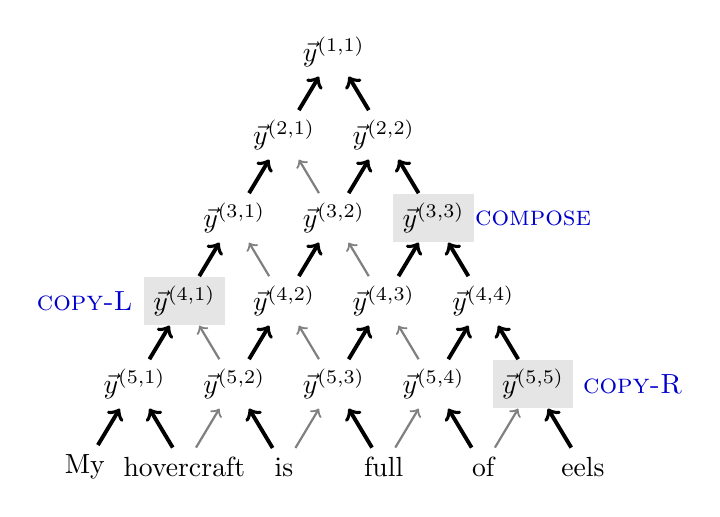
\begin{tikzpicture}
    \def\dx{18pt}
    \def\dy{30pt}
    \newcounter{i}
    \tikzstyle{highlight}=[fill=black!10]
    \tikzstyle{comment}=[color=blue!80!black]
    
    \stepcounter{i}\node  (\arabic{i}) at (0*\dx,6*\dy) {$\vec{y}^{(1, 1)}$};
    \stepcounter{i}\node  (\arabic{i}) at (-1*\dx,5*\dy) {$\vec{y}^{(2, 1)}$};
    \stepcounter{i}\node  (\arabic{i}) at (1*\dx,5*\dy) {$\vec{y}^{(2, 2)}$};
    \stepcounter{i}\node  (\arabic{i}) at (-2*\dx,4*\dy) {$\vec{y}^{(3, 1)}$};
    \stepcounter{i}\node  (\arabic{i}) at (0*\dx,4*\dy) {$\vec{y}^{(3, 2)}$};
    \stepcounter{i}\node[highlight]  (\arabic{i}) at (2*\dx,4*\dy) {$\vec{y}^{(3, 3)}$};
    \stepcounter{i}\node[highlight]  (\arabic{i}) at (-3*\dx,3*\dy) {$\vec{y}^{(4, 1)}$};
    \stepcounter{i}\node  (\arabic{i}) at (-1*\dx,3*\dy) {$\vec{y}^{(4, 2)}$};
    \stepcounter{i}\node  (\arabic{i}) at (1*\dx,3*\dy) {$\vec{y}^{(4, 3)}$};
    \stepcounter{i}\node  (\arabic{i}) at (3*\dx,3*\dy) {$\vec{y}^{(4, 4)}$};
    \stepcounter{i}\node  (\arabic{i}) at (-4*\dx,2*\dy) {$\vec{y}^{(5, 1)}$};
    \stepcounter{i}\node  (\arabic{i}) at (-2*\dx,2*\dy) {$\vec{y}^{(5, 2)}$};
    \stepcounter{i}\node  (\arabic{i}) at (0*\dx,2*\dy) {$\vec{y}^{(5, 3)}$};
    \stepcounter{i}\node  (\arabic{i}) at (2*\dx,2*\dy) {$\vec{y}^{(5, 4)}$};
    \stepcounter{i}\node[highlight]  (\arabic{i}) at (4*\dx,2*\dy) {$\vec{y}^{(5, 5)}$};
    \stepcounter{i}\node  (\arabic{i}) at (-5*\dx,1*\dy) {My};
    \stepcounter{i}\node  (\arabic{i}) at (-3*\dx,1*\dy) {hovercraft};
    \stepcounter{i}\node  (\arabic{i}) at (-1*\dx,1*\dy) {is};
    \stepcounter{i}\node  (\arabic{i}) at (1*\dx,1*\dy) {full};
    \stepcounter{i}\node  (\arabic{i}) at (3*\dx,1*\dy) {of};
    \stepcounter{i}\node  (\arabic{i}) at (5*\dx,1*\dy) {eels};
   
    \stepcounter{i}\node[comment]  (\arabic{i}) at (4*\dx,4*\dy) {\textsc{compose}};
    \stepcounter{i}\node[comment]  (\arabic{i}) at (-5*\dx,3*\dy) {\textsc{copy-L}};
    \stepcounter{i}\node[comment]  (\arabic{i}) at (6*\dx,2*\dy) {\textsc{copy-R}};
   
    \tikzstyle{extra} = [->, draw=black!50, line width=0.8pt]
    \tikzstyle{valid} = [->, draw=black, line width=1.4pt]

          \draw [valid] (2) -- (1);
          \draw [valid] (3) -- (1);
          
          \draw [valid] (4) -- (2);
          \draw [extra] (5) -- (2);
          \draw [valid] (5) -- (3);
          \draw [valid] (6) -- (3);
          
          \draw [valid] (7) -- (4);
          \draw [extra] (8) -- (4);
          \draw [valid] (8) -- (5);
          \draw [extra] (9) -- (5);
          \draw [valid] (9) -- (6);
          \draw [valid] (10) -- (6);
          
          \draw [valid] (11) -- (7);
          \draw [extra] (12) -- (7);
          \draw [valid] (12) -- (8);
          \draw [extra] (13) -- (8);
          \draw [valid] (13) -- (9);
          \draw [extra] (14) -- (9);
          \draw [valid] (14) -- (10);
          \draw [valid] (15) -- (10);
          
          \draw [valid] (16) -- (11);
          \draw [valid] (17) -- (11);
          \draw [extra] (17) -- (12);
          \draw [valid] (18) -- (12);
          \draw [extra] (18) -- (13);
          \draw [valid] (19) -- (13);
          \draw [extra] (19) -- (14);
          \draw [valid] (20) -- (14);
          \draw [extra] (20) -- (15);
          \draw [valid] (21) -- (15);
  \end{tikzpicture}

        \caption{The model structure used to compare \ii{turtle} and
          \ii{animal}.  Learned term representations are fed through
          either an NN or NTN comparison layer and then to a softmax
        classifier over the seven relations in Table~\ref{b-table}.}
  \label{sample-figure2}
\end{figure}

To compute the vector representation for a sentence, we populate the bottom row of the structure $\vec{y}^{(N,1...N)}$ with the embedddings of each of the words. We then compute the representations of each row starting at the second row from the bottom ($N - 1$), and moving from left to right. Computing one feature vector requires two steps. In the first step, a classifier produces a distribution $\vec{o}$ over the operations \{\textsc{copy-left, copy-right, compose}\}, and in the second step, that distribution is used to compute a feature vector $\vec{y}$.

To compute the distribution over operations at one node, $\vec{o}^{(i, j)}$, 




Choose an operation

row i
col j
amount of context C

To compute the vector representation for a sentence

\begin{equation} 
\label{TreeRNN}
\vec{o}^{(i,j)} = \text{softmax}(\mathbf{M_o} \colvec{7}
	{\vec{y}^{(i + 1, j - C + 1)}}
	{...}
	{\vec{y}^{(i + 1, j)}}
	{\vec{y}^{(i + 1, j + 1)}}
	{...}
	{\vec{y}^{(i + 1, j + C)}}
	{\vec{o}^{(i, j - 1)}}
	 + \vec{b}_o\,) \\
\end{equation}
	 
	 
\begin{equation}
\vec{y}^{(i,j)} = 
o^{(i, j)}_{1} \circ \vec{y^{(i + 1, j)}} +\\
o^{(i, j)}_{2} \circ \vec{y^{(i + 1, j + 1)}} +\\
o^{(i, j)}_{3} \circ \tanh(\mathbf{M_y} \colvec{2}{\vec{y}^{(i + 1, j)}}{\vec{y}^{(i + 1, j + 1)}} + \vec{b}_y)
\end{equation} 

For true relation $\rho$, and true operations $\omega^{(i,j)}$ for one example

\begin{equation}
loss = \lambda\theta^2-\ln(r_\rho) - \frac{1}{(N - 1)^2} \sum_{i = 1}^{N - 1} \sum_{j = 1}^{N - 1} \ln(o_{\omega^{(i,j)}})
\end{equation} 


\section{Discussion and conclusion}\label{sec:discussion}



data will be freely available

SICK presented an important challenge, we try to deliver on it.

aim to surpass sick in both size and label consistency

quote from SICK paper \cite{marelli2014sick}:

\begin{quote}
Not unreasonably, subjects found that, say, \ii{A woman is wearing an Egyptian headdress} does not contradict \ii{A woman is wearing an Indian headdress}, since one could easily imagine both sentences truthfully uttered to refer to a single scene where two different women are wearing different headdresses. In the future, a higher proportion of CONTRADICTION labels could be elicited by using grammatical and possibly visual cues (pictures) encouraging co-indexing of the entities in the two sentences.
\end{quote}

We use captions from the Flickr30k corpus \cite{hodoshimage} as the left hand side of each relation pair. That corpus ...

We randomly selected individual captions from that corpus to use in our own corpus, though in the interest of encouraging more complex source sentences without discarding too much source data, we downsample sentences with lengths of under 90 characters so that these sentences make up only half of our corpus, rather than the original 69\%.

... licencing ...

The instructions for this phase were integrated into the design of the data collection interface. The text of those instructions is shown in Figure~\ref{instructions-1}. We chose to use three classes, corresponding to ENTAILMENT, CONTRADICTION, and NEUTRAL classes used in SICK.

\begin{figure}
\footnotesize
% \toprule
The Stanford University NLP Group is collecting data for use in research on computer understanding of English. We appreciate your help!

We will show you the caption for a photo. We will not show you the photo. Using only the caption and what you know about the world:
\begin{itemize}
\item Write one alternate caption that is \textbf{definitely} a \textbf{true} description of the photo. \ii{Example: For the caption "Two dogs are running through a field." you could write "There are animals outdoors."}
\item Write one alternate caption that \textbf{might be} a \textbf{true} description of the photo. \ii{Example: For the caption "Two dogs are running through a field." you could write "There are animals outdoors."}
\item Write one alternate caption that is \textbf{definitely} a \textbf{false} description of the photo. \ii{Example: For the caption "Two dogs are running through a field." you could write "There are animals outdoors." This is different from the maybe correct category because its impossible for the dogs to be both running and sitting.}
\end{itemize}
\textbf{Problems} (optional)   If something is wrong with the caption that makes it difficult to understand, do your best above and let us know here.
% \bottomrule
\caption{\label{instructions-1}Examples of training data from the newly collected entailment corpus.}
\end{figure}


We posted 15.5k ImageFlickr captions. We showed each of the first 10k captions to five workers, yielding fifteen reponse sentences per source caption, with five assigned to each of the three labels. Then, to ensure maximal diversity in the test set, we showed the remaining 5.5k source captions to one worker each,  yielding only three responses per source caption.

We collected 143,023 pairs, after excluding less than 100 worker responses in which the worker reported that they could not understand the source caption, or in which a field was accidentally left blank. The average worker response sentence was 7.8 words long. 1100 workers participated in the task.

pre-verification distribution:

Recompute after removing blanks:
29305 contra
29304 neut
29305 ent

% ditto examples
%
\begin{table*}
  \centering\footnotesize
  \begin{tabular}{p{6.5cm}cp{6.5cm}}
  \toprule
A busy street with building lined up and people walking down the street outside and nighttime. &\ii{entailment}	&People lined up\\
\rule{0pt}{3ex}Two men stand in an electric outdoor lift. &\ii{neutral}	& The two men are inspectors for the FDA, waiting to inspect the second level of the pharmaceutical plant.\\
\rule{0pt}{3ex}A young redheaded girl, wearing a yellow shirt, black pants, and sneakers, jumping in a grassy field with blue skies and wispy clouds in the background. &\ii{entailment}	& A girl jumps in a grassy field\\
\rule{0pt}{3ex}A crowd of people, one with a guitar, are standing in the street under the 7th Avenue street sign. &\ii{neutral}	& The crowd listening to the man play guitar.\\
\rule{0pt}{3ex}A woman wearing bike shorts and a skirt is riding a bike and carrying a shoulder bag.  &\ii{contradiction}& A woman driving a car.\\
    \bottomrule
  \end{tabular}
  \caption{\label{examplesofscedata}The instructions presented to workers during data collection.}
\end{table*}


% Screenshot from phase 1


% Screenshot from phase 2

The data is freely available at (POST DATA), and is released under a CreativeCommons
Attribution-ShareAlike licence, which is the same licence used for the Flickr30k source captions.

\paragraph{validation}

The majority of the sentence pairs in the corpus have not been reviewed by anyone since their construction as part of the data collection Mechanical Turk task, except to remove blank responses and responses where the original author flagged the source caption for review. However, in order to measure the accuracy of our corpus, and in order to improve the quality of our test and development sets, we did perform an additional round of validation for TODOk examples.

This validation phase is not fundamentally different from the Mechanical Turk labeling task used for the SICK entailment data: we present workers with pairs of sentences (in our case, in batches of five per screenfull), and ask them to choose a single label for each pair. We supplied each pair to four annonators, yielding five labels per pair including the label used by the original composer of the pair. 

TODO: Data filtering? Data re-labeling?

\begin{figure}
\footnotesize
%\toprule
TODO: VALIDATION INSTRUCTIONS
%\bottomrule\\

\caption{\label{instructions-2}The instructions presented to workers during data validation.}
\end{figure}

\paragraph{data partition}

\paragraph{simple baselines}

MFC

BLEU

Summing + NN


\subsubsection*{Acknowledgments}

We thank ...

Grant acknowledgments for money?

%%%

% \section*{Acknowledgments}

% Do not number the acknowledgment section.

\bibliographystyle{acl}
\bibliography{MLSemantics} 

\end{document}
